\documentclass{aamas2013}

\usepackage{amssymb}
\usepackage{graphicx}
\usepackage{epstopdf}
\usepackage{multirow}
\usepackage{url,eqnarray,amsmath,amssymb,epsfig,verbatim}
\usepackage{tikz}
\usepackage{subfig}
\usepackage{booktabs}
\usetikzlibrary{matrix,arrows,decorations.pathmorphing,backgrounds,shadows,positioning}
\pdfpagewidth=8.5truein
\pdfpageheight=11truein

\providecommand{\customsubsub}[1]{~\\[-0.7em]\noindent{\bf {#1.}}}
%%some notation
\providecommand{\E}{\mathbb{E}}
\providecommand{\SALEP}{SALE POMDP}
\providecommand{\NoAQ}{\textsc{NoAQ}}
\newlength{\EqSpace}
\setlength{\EqSpace}{-9mm}


\makeatletter
 \let\@copyrightspace\relax
 \makeatother
\begin{document}


\title{A POMDP Based Approach to Optimally Select Sellers in E-Marketplaces}

\author{Paper XXX}

\maketitle

\begin{abstract}
In e-marketplaces, buying agents choose among multiple sellers, finding the best one to perform a transaction. A seller's quality is mainly determined using buyers' assessments on the seller based on previous transactions. How a buyer utilizes existing information and chooses the right seller, while maximizing its utility derived from the decision process is crucial, since the value derived from a successful transaction with the seller, may be negligible relative to the cost of choosing the right seller. This paper presents \SALEP{}, a framework based on the \textit{Partially Observable Markov Decision Process}, which helps a buyer to optimally select the right seller to perform a transaction. The framework is robust in the sense that it also allows to reason about the quality of other buying agents (advisors) in the market, who provide opinions about the sellers. Experimental results on the ART Testbed demonstrate that \SALEP{} can optimally select the right sellers and advisors (to ask opinions), effectively balancing the trade-off between the cost of obtaining and benefit of more information, than traditional trust models.
\end{abstract}

\category{I.2.11}{Distributed Artificial Intelligence}{Intelligent Agents; Multiagent Systems}

\terms{Performance; Design}

\keywords{Seller Selection, E-Marketplace, POMDPs.}

\section{Introduction}\label{introduction}

In multi-agent based e-marketplaces, self-interested selling agents can act maliciously by not delivering products with the same quality as promised. It is thus important for buying agents to analyze the quality of sellers and determine which sellers to do business with. Buyers maintain beliefs over the quality levels of the sellers, based on their previous transactions with the seller, using which they can select the best seller to interact. However, realistically, in most e-marketplaces, buyers often encounter sellers with which they have no previous experience. In such cases, they can query other buyers (called advisors) about their beliefs on the sellers' quality.

A number of trust models (\textit{e.g.} BRS~\cite{whitby05}, TRAVOS~\cite{teach06}, Personalized~\cite{zhang09thesis}, BLADE~\cite{regan2006bayesian}, etc.), have been proposed by researchers in the multi-agent community to help buyers assess seller quality and choose business partners. These approaches work by combining the buyer's own belief and those of the advisors, to estimate the true quality of the seller. However, the above approaches mainly focus on accurately estimating the quality of the seller rather than optimally choosing a right seller to perform transaction with. They do not consider the underlying trade-off between the cost of estimating seller's quality and the value derived from a successful transaction with the seller. This is because the above trust models fail to reason \textit{when} it is necessary to query advisors, though they may determine \textit{whom} to query by analyzing the quality levels (trustworthiness) of the advisors who provide accurate opinions\footnote{opinion refers to the advisor's belief on the seller} about the sellers. Most approaches simply query all advisors whom they consider honest. This will in fact result in negligible utility for the buyer, especially when the querying advisors are large in numbers, since the cost of querying advisors may be greater than the value derived from a successful transaction with the seller. Rather than querying all potential advisors, the buying agent may query advisors until it is sufficiently sure that it has identified a seller with the expected quality. This is a strong motivation behind our work where we consider the seller selection problem as a decision problem, resolving the trade off between the cost of selecting the right seller and the value derived from the transaction with the seller.

POMDPs provide such a framework for making optimal decisions in partially observable environments, where an agent cannot directly observe the underlying state. A POMDP agent works towards the main goal of maximizing the expected discounted future reward~\cite{kaelbling1998planning} (buyers' utility in our case). Modeling the buying agent as a POMDP will help to optimally select the right seller (rather than accurately determining the quality of the sellers). Regan \textit{et al.}~\cite{regan2005advisor} proposed the \textit{Advisor} POMDP, which also considered the seller selection problem as a \textit{Partially Observable Markov Decision Process}. However, their approach did not reason about advisors' quality levels and considered all advisors to be trustworthy. Thus, \textit{Advisor} POMDP cannot cope with unfair rating attacks~\cite{irissappane2012towards}, where advisors may provide incorrect opinions about the sellers. Also, in \textit{Advisor} POMDP, each advisor provides opinions about its beliefs on all sellers, when queried, resulting in a lot of unnecessary information. However, rather than estimating the quality of all sellers, the only goal should be to select the seller with high quality.

In this paper, we present the detailed analysis of \emph{(S)eller \& (A)dvisor se(LE)ction POMDP (\SALEP)}~\cite{oliehoekreasoning}. \SALEP\ models the buying agent as a POMDP, with the main goal of optimally selecting the right seller to perform a transaction. In this process, it maintains the beliefs over the quality levels of the sellers, as well as that of the advisors. To query advisors about the quality of the sellers, it firstly determines the quality of the advisors, thereby limiting its interactions to the honest ones. It also makes  provision to query advisors about their beliefs on other advisors, sufficiently using it to improve its own beliefs and make optimal decisions. We also analyze how \SALEP\ can be extended to be more usable in e-market scenarios, effectively dealing with the seller selection problem in a holistic manner than the traditional trust models. Specifically, we have: 1) modeled \SALEP\ as a \textit{factored} POMDP, to resolve the scalability issues, which is a limiting factor in solving most POMDPs~\cite{poupart2005exploiting}; 2) modeled the advisor behavior  (in providing unfair ratings) to be more realistic. Specifically two types of attacking behavior are considered, dishonest advisors who exhibit \textit{random} behavior in providing opinions about other agents and those who behave in an \textit{adversarial} manner, providing complementary opinions; 3) allowed to consider the influence of previous responses (history) in the POMDP formulation and 4) performed a thorough evaluation of the \SALEP\ model using the ART Testbed, comparing its effectiveness against other trust models.


The rest of the paper is organized as follows. Section~\ref{sec:2} gives a brief discussion of related work and continues to argue the importance and uniqueness of the \SALEP\ framework. The detailed description of the \SALEP\ model is present in Section~\ref{sec:3}. In Section~\ref{sec:4}, we demonstrate how \SALEP\ is can be modeled as a \textit{factored} POMDP. In Section~\ref{sec:5}, through extensive experimentation on the ART testbed, we demonstrate the effectiveness of \SALEP\ in optimally selecting the right sellers to perform transaction. The scalability of the \textit{factored} approach and methods to improve the robustness of the \SALEP\ model are also discussed. Finally, Section~\ref{sec:5} concludes the current work and proposes future work.

\section{Related Work}\label{sec:2}


Many trust models have been proposed in literature to address the seller selection problem. They model sellers' quality (reputation), using opinions from other buyers and thereby select the best seller to interact with. The Beta Reputation System (BRS)~\cite{whitby05} models the seller's reputation as the expected value of the beta probability distribution of the trusted advisors' beliefs about the seller. If the calculated reputation of a seller based on the opinions from the set of honest buyers falls within the rejection area ($q$ quantile or $1-q$ quantile) of the beta distribution of an advisor's beliefs on the seller, then the advisor is considered untrustworthy. BRS is a centralized approach and is heavily based on the \textit{majority rule}. Teacy \emph{et al.}~\cite{teach06} propose TRAVOS which is also based on beta probability distribution. To calculate the reputation of a seller, it integrates buyer's own beliefs about sellers as well as the beliefs of advisors, after assessing their credibility. The personalized approach~\cite{zhang08}, models seller's quality as a weighted score of its public and private reputation. The private reputation is calculated as the expected value of the beta probability distribution of the buyer's beliefs on the seller and the public reputation is calculated using the beliefs of the advisors, after discounting them based on their trustworthiness. However, it assumes the behavior of the advisors to be consistent across all sellers.

The BLADE approach of Regan et al.~\cite{regan2006bayesian} applies Bayesian learning to reinterpret advisors' beliefs instead of filtering them. The BLADE model allows a buyer to learn other advisors' evaluation functions on different features of the services delivered by sellers, by analyzing their beliefs. This makes it possible to adjust the advisor's beliefs, thereby coping with subjectivity and deception, while determining the quality of the seller. However, the model assumes consistent advisor behavior and also requires multiple transactions with the same seller to accurately interpret its quality. In contrast, in \SALEP\ we learn about advisors by asking other advisors, thereby avoiding the need to engage in costly transactions. Also, all the above trust models do not provide optimal decision making for the buyer on whether and from which seller to perform transaction, which is exactly what our approach tries to offer.

Few works based on POMDPs exist to address the seller selection problem using the notion of trust. The \textit{Advisor} POMDP~\cite{regan2005advisor}, described by $\left\langle \mathcal{S},\mathcal{A},\mathcal{T},\mathcal{R},\Omega,\mathcal{O}\right\rangle$, where $\mathcal{S}$ represents the possible states consisting of the seller's quality and the outcome of the transaction with seller, $\mathcal{A}$ represents the actions $\in {ask, buy}$, $\mathcal{T}$ represents the transition functions, $\mathcal{R}$ represents the rewards based on the outcomes of the transaction, $\Omega$ represents the observations from advisors, consisting of the advisors' beliefs about the sellers along with the certainty and $\mathcal{O}$ denotes the observation function, updates its belief about the seller via Bayes' rule, on interacting with other advisors in the environment, thereby selecting the right seller to perform transaction. However, \textit{Advisor} POMDP does not consider advisor's quality to be a part of the state space, making it vulnerable to unfair rating attacks. Also the observations in \textit{Advisor} POMDP contain beliefs about all sellers, resulting in an unnecessary exchange of information during the $ask$ actions. Seymour \textit{et al.}~\cite{seymour2009trust} proposed TI-POMDP, which adds trust modeling to the I(interactive)-POMDP framework~\cite{gmytrasiewicz2005framework}. I-POMDP is a multi-agent extension of the POMDP framework, in which each agent maintains beliefs about both the physical states of the world and the decision process models of the other agents. The TI-POMDP maintains the basic components of the I-POMDP, and adds trust modeling as a primary decision factor for the agents. In addition to the state belief model, an agent maintains and updates a trust model (a rating of the trustworthiness of the other agents) for the environment. This trust model contains an agent's level of trust in the other agents, which helps to decide whether or not to cooperate with another agent on a given task. However, this model depends heavily on communication between the agents for decidability~\cite{mayo2010multi}. Whereas, in our work, we aim to optimally select the sellers, under conditions of uncertainty, by securing additional information on the seller's (and advisor's) quality levels from other agents in the market, eliminating the need to explicitly engage in personal interactions with the sellers.

\section{The \SALEP{} Model}\label{sec:3}

In this section, we introduce the \SALEP{} framework for dealing with the seller section problem by optimally selecting the right seller to perform transaction. Unlike \textit{Advisor} POMDP, \SALEP{} assumes that advisors also have quality levels (\emph{trustworthiness}) and considers it as part of the state space. It also allows agents to query about the quality of other advisors in the system. Each \SALEP{} agent is described using the following elements.
\begin{itemize}
\item $\mathcal{S}$---a set of possible states of the environment. A state contains the quality levels\footnote{we assume discrete quality levels, in order to use standard POMDP solvers.} of each seller, advisor and the status of the current transaction. Let $\mathcal{Q}$ be the discrete set of seller quality levels and $\mathcal{U}$ be the set of advisor quality levels. Then, a state is a tuple $s=\left\langle \vec{q},\vec{u},sat\right\rangle $, where $\vec{q}\in\mathcal{Q}^{J}$ is a vector indicating the quality of each seller, $\vec{u}\in\mathcal{U}^{I}$ a vector indicating the quality of each advisor, and $sat\in\left\{ -1,0,+1,+2\right\} $ indicates whether the outcome of a transaction is satisfactory $(+1)$, unsatisfactory $(-1)$, given up $(+2)$ due to the $donotbuy$ action or whether no transaction took place yet $(0)$. We also write $q_{j}$ for the $j$-th element of $\vec{q}$ and $u_{i}$ for the $i$-th element of $\vec{u}$. The end of the decision process (after a buy/donotbuy action) is modeled using sets of \textit{terminal states}. That is, a terminal state is a state where $sat=+1$, $sat=+2$ or $sat=-1$. We will consider these sets of states as single states called \textit{satisfied}, \textit{unsatisfied} and \textit{gaveup}.

\item $\mathcal{A}$---a set of actions which can be:\\[-1.8em]
        \begin{itemize}
            \item $seller\_query_{ij}$, ask advisor $i$ about seller~$j$,
            \item $advisor\_query_{ii'}$, ask advisor $i$ about advisor~$i'$,
            \item $buy_{j}$, buy from seller~$j$.
            \item $do\_not\_buy$, decide not to buy from any seller.
        \end{itemize}
    \vspace{-1em}
\item $T$---a transition function that specifies $\Pr(s'|s,a)$, the probability of transferring to a state $s'$ given that action $a$ was taken in state $s$. We assume that when taking a query action, the state does not change:
        \begin{equation}
            \forall_{i,j}\quad\Pr(s'|s,seller\_query_{ij})=\delta_{ss'}
        \end{equation}
        \\[\EqSpace]
        \begin{equation}
            \forall_{i,i'}\quad\Pr(s'|s,advisor\_query_{ii'})=\delta_{ss'}
        \end{equation}
    $\delta_{ss'}$ is the Kronecker delta \textit{i.e.} $1$ if and only if $s=s'$. When taking a $buy_{j}$ action, the state will always transition to a terminal state. The transition probabilities to terminal states give a definition of the quality levels. In general, chances of transition to \textit{satisfied} should be higher when buying from higher quality sellers. Together, the specifications of these transitions imply the assumption that quality and trust-levels are stationary for the duration of the decision process.

\item $R$---a reward function specifying $R(s,a,s')$: a small cost is associated with ask action $R(s,seller\_query_{ij})=R(s,advisor\_query_{ii'})=R_{ask}$; a reward is associated with a good purchase $R(s,buy_j,s'=\left\langle \vec{q},\vec{u},sat=+1\right\rangle )=R_{sat}$; a penalty is levied when the outcome of a transaction is \emph{unsatisfied} $R(s,buy_j,s'=\left\langle\vec{q},\vec{u},sat=-1\right\rangle )=R_{unsat}$ and a penalty for taking the $do\_not\_buy$ action when in fact there is a seller of high enough quality (we use $-R_{sat}$), otherwise the reward for this action is $0$. Once the state changed to \textit{satisfied}, \textit{unsatisfied} or \textit{gaveup}, no further rewards are given.
\item $\Omega$---a set of observations. When a \emph{query} action is performed the agent will receive an observation from the set of discriminated quality levels. That is, after a $seller\_query_{ij}$ action, the agent receives an observation $o\in\mathcal{Q}$ corresponding to the quality of seller $j$, while after an $advisor\_query_{ii'}$ it will get an observation $o\in\mathcal{U}$ corresponding to the quality of advisor $i'$. When the agent transitions to a terminal state, it receives the observation \textit{ended}. As such $\mathcal{O}=\mathcal{Q}\cup\mathcal{U}\cup\left\{ ended\right\} $.
\item $O$---the observation function that specifies $\Pr(o|a,s)$. As in the Advisor POMDP, there is no a priori correct way to specify the observation probabilities. The probabilities picked for the observation function define the meaning of different trust levels. In general, the idea is that trustworthy advisors will give more accurate and consistent answers than untrustworthy ones.
\item $b^{0}$---the initial state distribution. It is dependent on the subjective beliefs of the agent, when the need for purchasing an item arises. For simplicity, one may start with a uniform belief over the quality levels, but a different initial belief can also be obtained as a result of previous interactions. That is, once the $buy_j$ or $do\_not\_buy$ action is performed, the resulting belief can be used as the basis for an initial belief for a new seller selection instantiation. In a bit more detail, There are two sources of previous experience: 1) previous seller selection tasks: the modified belief state resulting from advice in a previous problem can be retained and 2) actual experiences with sellers: even though in the decision making task we model a transition to a terminal state with a deterministic \emph{ended} observation, the actual order will result in the owner of the agent being satisfied or not and this information can be used to update the final belief of the agent's previous seller selection task giving a new initial belief for a new task\footnote{In fact this can be an important mechanism to deal with advisors that are consistent but deceptive and settings in which the majority of advisors is untrustworthy.}
\item $h$---the \emph{horizon} of the problem. That is the number of time steps, or \emph{stages}, for which we want to plan. We will assume that $h$ is infinite in this paper.
\end{itemize}
When the \SALEP{} agent interacts with the environment, it maintains a \emph{belief} $b$, i.e., a probability distribution over states via Bayes' rule. That is, when $b(s)$ specifies the probability of $s$ (for all $s$), we can derive $b'$ an updated belief after taking some action~$a$ and receiving an observation~$o$.  The belief updates are performed such that they correlate the state factors in meaningful ways. For instance, observing good after $seller\_query_{ij}$ should give more weights to states where the seller is high quality $q_j = H$ and the advisor is trustworthy $u_i = T$, and less weights to states where the seller is low quality $q_j = L$ and the advisor is untrustworthy $u_i = U/A$.  Similarly, observing $T$ after $advisor\_query_{ii'}$ should put more weight on states where $u_i' = T$ and $u_i = T$, and decrease weight on states where $u_i' = U/A$ and $u_i = T$. Assuming discrete sets of states and observations, this update can be written as follows:
\begin{equation}
b'(s')\hspace{-1mm}=\hspace{-1mm}\frac{ \Pr(s',o|b,a) } {\Pr(o|b,a)}\
\hspace{-1mm}=\hspace{-1mm}\frac{1}{ \Pr(o|b,a) }
\Pr(o|a,s')
\sum_s
\Pr(s'|s,a)
b(s)
\label{eq:BU}
\end{equation}\\[-2mm]
Here, $\Pr(o|b,a)$ is a normalization factor. 
%%SAVESPACE
%Regan et al.~\cite{Regan05PST} give a step by step illustration of the belief
%update in the continuous state case.

These beliefs are the basis for decision making: a policy $\pi$ maps beliefs to actions
$\pi(b)=a$. The goal of solving the POMDP is to find an optimal
policy that maximizes the expected discounted cumulative reward, also called
\emph{value}:\\[-2mm]
\begin{equation}
V(\pi)=\E\Big[\sum_{t=0}^{h-1} \gamma^t R(s,a,s') \mid \pi,b^0\Big],
\end{equation}\\[-3mm]
with $0\leq\gamma<1$ the discount factor.

Finding an optimal policy $\pi^*$ is intractable in general (PSPACE complete \cite{papadimitriou1987complexity}), however, in recent years substantial advances
have been made in approximate solutions (e.g.,~\cite{kurniawati2008sarsop,silver2010monte}). Since the \SALEP{} really is a \emph{factored} POMDP, we try and use solvers that exploit this property such as symbolic Perseus \cite{poupart2005exploiting} as described in the next section.

\section{Factored Representation}\label{sec:4}

POMDPs with very large state spaces are impractical to be solved by the classic solution algorithms. However, such state spaces can be described using a set of state variables, and the effects of actions in terms of their effects on these variables. Dynamic Bayesian Networks (DBNs) with conditional probability tables (CPTs) in the form of decision-trees or
graphs are often used to represent these effects compactly referred to as a \textit{factored} representation~\cite{shani2013task}. Solvers such as Symbolic Perseus~\cite{poupart2005exploiting} exploit this \textit{factored} structure to resolve scalability issues in POMDPs.

To illustrate the \textit{factored} nature of the \SALEP{}, we will consider a simple case of the seller selection problem with $1$ seller and $2$ advisors such that $\mathcal{Q}=\left\{ L,H\right\} $ denoting $L$(ow) and $H$(igh) seller quality and $\mathcal{U}=\left\{ T,U, A\right\} $ denoting $T$(rustworty), $U$(ntrustworty) or $A$(dversarial) advisor quality levels. Here each state $s \in \mathcal{S}$ is a compilation of the quality of each seller, quality of each advisor and transaction outcome, \textit{i.e.} $s=\left\langle \left\langle q_1\right\rangle, \left\langle u_1, u_2\right\rangle, sat\right\rangle$. To factor the \SALEP{} model, we decompose the transition and observation functions as follows.\\
 \textbf{Buy Action} The DBN and CPT for the $buy_{1}$ action  (buy from $s_1$) are shown in Fig~\ref{fig:BuyS1}. The probability of transferring to a state $s'$ given that action $buy_{1}$ was taken in state $s$ can be factored into a product of smaller conditional distributions with respect to its parent variables as shown in Eqn.~\ref{eq:buy}.  $\Pr(sat'|q'_1,sat,buy_{1})$ signifies that the outcome of a transaction $sat'$ at a time step depends on the previous status of the transaction $sat$, the true quality of the seller $s'_1$ and the $buy_{1}$ action. The CPT for $sat'$ variable is framed assuming that buying from a high quality seller will lead to \emph{satisfied} with 80\% probability: $ \Pr(sat=-1|\left\langle sat=0,q_{j}=L\right\rangle ,buy_{j})=0.8$. Similarly, we will assume that a low quality seller will lead to \emph{unsatisfied} with probability $0.8$. For the $do\_not\_buy$ action, the outcome $sat'$ is not dependant on the seller quality $q'_1$ and $\Pr(sat'|sat,do\_not\_buy)=1$.\\
\vspace{-2mm}
 \begin{equation}
\begin{split}
\Pr(s'|s,buy_{1}) & = \Pr(u'_1,u'_2, q'_1,sat'|u_1,u_2,q_1,sat,buy_{1}) \\
& =  \Pr(u'_1|u_1,buy_{1})\times \Pr(u'_2|u_2,buy_{1}) \times \\
& \hspace{3.5mm}\Pr(q'_1|q_1,buy_{1}) \hspace{-0.5mm}\times\Pr(sat'|sat,q'_1,buy_{1})
\end{split}
 \label{eq:buy}
\end{equation}
 \textbf{Seller Query} Fig~\ref{fig:AskA1S1} shows the DBN and CPT for the action $seller\_query_{11} (sq_{11})$ (query $a_1$ about $s_1$).  Eqn~\ref{eq:sellerquery} shows that observing the quality of a seller $s_1$ through $o'$ is conditionally dependant on the current quality of the seller $q'_1$ (after the $seller\_query_{11}$ action) and the quality of the advisor $u'_1$, who provides opinion. $2$ possible observations are considered: $good$ (i.e., the advisor says that the seller is high quality) denoted by \textit{g} and $bad$ (the seller is said to be low quality) denoted by \textit{b}.  The observation probabilities for the $seller\_query_{ij}$ action are such that asking a trustworthy (T) advisor gives more accurate observations, while untrustworthy ones may provide a random (U) opinion or they can be adversarial (A) in nature.  We will obtain a similar figure for $seller\_query_{21}$ action.\\
 \vspace{-5mm}
 \begin{figure}[h!]
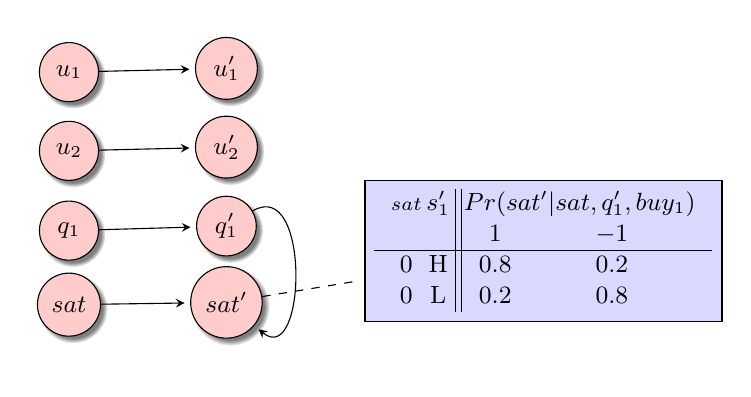
\begin{tikzpicture}[>=stealth,->,shorten >=2pt,looseness=.5,auto]
\matrix [matrix of math nodes,
column sep={20mm,between origins},
row sep={10mm,between origins},
nodes={circle, circular drop shadow, draw, minimum size=7.5mm, fill=red!20, font=\small}]
{
|(u_1)| u_1 & |(u'_1)| u'_1 \\
|(u_2)| u_2 & |(u'_2)| u'_2 \\
|(q_1)| q_1 & |(q'_1)|q'_1\\
|(sat)| sat & |(sat')| sat' \\
};
\node (some) at (5,-0.8) [draw, fill=blue!15,font=\small] {
\begin{tabular}{c@{\hspace{0.6mm}}c@{\hspace{0.6mm}}||c@{\hspace{0.6mm}}c@{\hspace{0.6mm}}}
     % \multicolumn{2}{c}{t}&\multicolumn{2}{c}{t+1}\\
     \centering
     \scriptsize
     \textbf{$sat$}&\textbf{$s'_1$}&\multicolumn{2}{@{\hspace{0.2mm}}c}{$Pr(sat'|sat,q'_1,buy_1)$}\\
     && \textbf{$1$} & \textbf{$-1$}\\
    \hline
     0 &H & 0.8 & 0.2 \\
    0&L & 0.2 & 0.8 \\
    \end{tabular}
    \hspace{-1mm}
};
\begin{scope}[every node/.style={font=\small\itshape}]
\draw (u_1)--(u'_1);
\draw (u_2)--(u'_2);
\draw (q_1)--(q'_1);
\draw (sat)--(sat');
\draw (q'_1)to [bend left, relative, out=120, in=50, looseness=1.5](sat');
\draw [-,dashed](sat')--(some);
%\draw (D) to [bend right, looseness=1]
%node [near start] {b} node [near end] {e} (A);
\end{scope}
\end{tikzpicture}
\caption{DBN for $buy_{1}$} \label{fig:BuyS1}
\end{figure}
 \vspace{-5mm}
 \begin{figure}[h!]
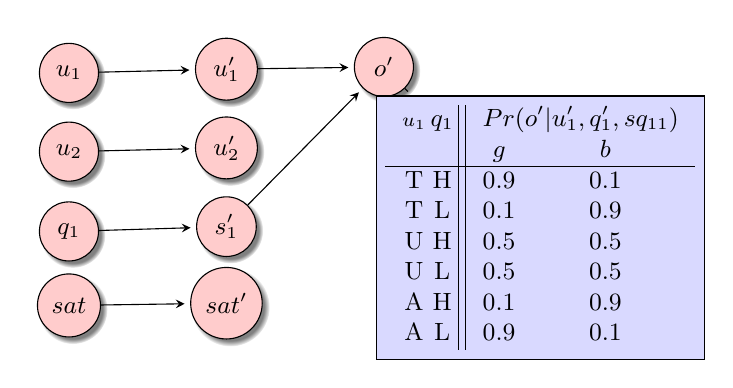
\begin{tikzpicture}[>=stealth,->,shorten >=2pt,looseness=.5,auto]
\matrix [matrix of math nodes,
column sep={20mm,between origins},
row sep={10mm,between origins},
nodes={circle, circular drop shadow, draw, minimum size=7.5mm, fill=red!20, font=\small}]
{
|(u_1)| u_1 & |(u'_1)| u'_1  &|(o')| o'\\
|(u_2)| u_2 & |(u'_2)| u'_2 \\
|(q_1)| q_1 & |(q'_1)| s'_1\\
|(sat)| sat & |(sat')| sat' \\
};
\node (some) at (4,-0.5) [draw, fill=blue!15,font=\small] {
\begin{tabular}{c@{\hspace{0.6mm}}c@{\hspace{0.6mm}}||c@{\hspace{0.6mm}}c@{\hspace{0.6mm}}}
     % \multicolumn{2}{c}{t}&\multicolumn{2}{c}{t+1}\\
     \centering
     \scriptsize
       \textbf{$u_1$}& \textbf{$q_1$} &\multicolumn{2}{c}{$Pr(o'|u_1',q_1',sq_{11})$}\\
     && \textbf{$g$} & \textbf{$b$}\\
      \hline
     T &H & 0.9 & 0.1 \\
     T&L & 0.1 & 0.9 \\
     U &H & 0.5 & 0.5 \\
     U & L & 0.5 & 0.5\\
     A &H & 0.1 & 0.9 \\
     A & L & 0.9 & 0.1\\
    \end{tabular}
};
\begin{scope}[every node/.style={font=\small\itshape}]
\draw (u_1)--(u'_1);
\draw (u_2)--(u'_2);
\draw (q_1)--(q'_1);
\draw (sat)--(sat');
\draw (q'_1)--(o');
\draw (u'_1)--(o');
\draw [-,dashed](o')--(some);
%\draw (D) to [bend right, looseness=1]
%node [near start] {b} node [near end] {e} (A);
\end{scope}
\end{tikzpicture}
\caption{DBN for $seller\_query_{11}$} \label{fig:AskA1S1}
\end{figure}
 \vspace{-5mm}
 \begin{figure}[h!]
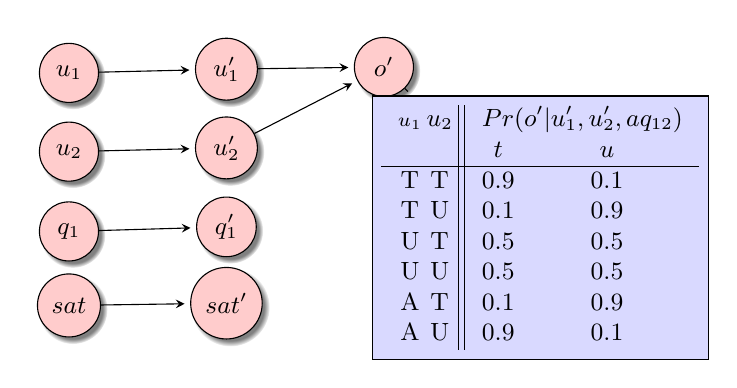
\begin{tikzpicture}[>=stealth,->,shorten >=2pt,looseness=.5,auto]
\matrix [matrix of math nodes,
column sep={20mm,between origins},
row sep={10mm,between origins},
nodes={circle, circular drop shadow, draw, minimum size=7.5mm, fill=red!20, font=\small}]
{
|(u_1)| u_1 & |(u'_1)| u'_1  &|(o')| o'\\
|(u_2)| u_2 & |(u'_2)| u'_2 \\
|(q_1)| q_1 & |(q'_1)| q'_1\\
|(sat)| sat & |(sat')| sat' \\
};
\node (some) at (4,-0.5) [draw, fill=blue!15,font=\small] {
\begin{tabular}{c@{\hspace{0.6mm}}c@{\hspace{0.6mm}}||c@{\hspace{0.6mm}}c@{\hspace{0.6mm}}}
     % \multicolumn{2}{c}{t}&\multicolumn{2}{c}{t+1}\\
     \centering
     \scriptsize
       \textbf{$u_1$}& \textbf{$u_2$} &\multicolumn{2}{c}{$Pr(o'|u_1',u_2',aq_{12})$}\\
     && \textbf{$t$} & \textbf{$u$}\\
      \hline
     T &T & 0.9 & 0.1 \\
     T&U & 0.1 & 0.9 \\
      U&T & 0.5 & 0.5 \\
     U & U & 0.5 & 0.5\\
     A &T & 0.1 & 0.9 \\
     A & U & 0.9 & 0.1\\
    \end{tabular}
};
\begin{scope}[every node/.style={font=\small\itshape}]
\draw (u_1)--(u'_1);
\draw (u_2)--(u'_2);
\draw (q_1)--(q'_1);
\draw (sat)--(sat');
\draw (u'_1)--(o');
\draw (u'_2)--(o');
\draw [-,dashed](o')--(some);
%\draw (D) to [bend right, looseness=1]
%node [near start] {b} node [near end] {e} (A);
\end{scope}
\end{tikzpicture}
\caption{DBN for $advisor\_query_{12}$} \label{fig:AskA1A2}
\end{figure}
 \begin{equation}
 \centering
\begin{split}
\Pr(o'|s,sq_{11})& =\Pr(o'|u_1',u_2',q_1',sat',sq_{11})\\
& =\Pr(o'|u_1',q_1',sq_{11})
\end{split}
 \label{eq:sellerquery}
\end{equation}
\textbf{Advisor Query} Fig~\ref{fig:AskA1A2} shows the DBN and CPT for the action $advisor\_query_{12} (aq_{12})$ (query $a_1$ about $a_2$).  Eqn~\ref{eq:advisorquery} show that observing the quality of advisor $a_2$ using the variable $o'$ (we use the same observation variable for simplicity) is conditionally dependant on the current quality of the advisor $u'_2$ (after the $advisor\_query_{12}$ action) and the quality of the advisor $a_1$ ($u'_1$), who provides opinion. We will obtain a similar figure for $advisor\_query_{21}$ action.
\begin{equation}
\begin{split}
\Pr(o'|s,aq_{12})&=\Pr(o'|u_1',u_2',s_1',sat',aq_{12})\\
&=\Pr(o'|u_1',u_2',aq_{12})
\end{split}
 \label{eq:advisorquery}
\end{equation}
The conditional probability tables in the above figures can be further compressed by exploiting context-specific independence which refers to the fact that some random variables are independent of each other in some contexts (i.e., for some specific values of other random variables). In general, context-specific independence allows one to compactly represent probability and utility tables using Horn rules [107] decision trees (DTs) or algebraic decision diagrams (ADDs)~\cite{boutilier1996context}. We will show one such ADD for the CPT in Fig~\ref{fig:AskA1S1}. 
 \begin{figure}[h!]
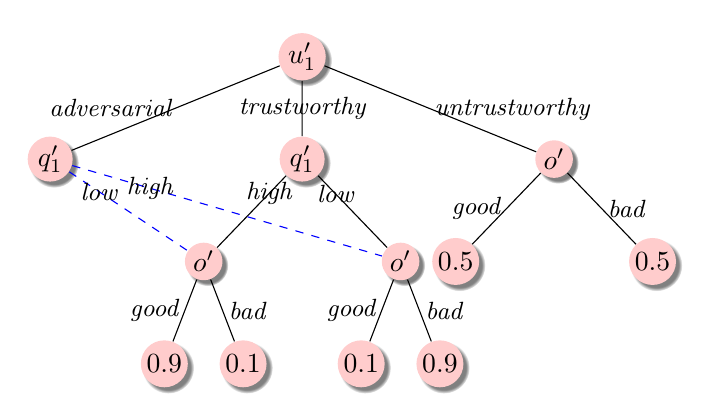
\begin{tikzpicture}
[level distance=13mm,
every node/.style={fill=red!20,circle,inner sep=1pt},
level 1/.style={sibling distance=32mm,nodes={fill=red!20}},
level 2/.style={sibling distance=25mm,nodes={fill=red!20}},
level 3/.style={sibling distance=10mm,nodes={fill=red!20}}]
\node [circular drop shadow] {$u'_1$}
child {node (AS) [circular drop shadow] {$q'_1$}
edge from parent
node[left,draw=none,fill=none,font=\small\itshape] {adversarial}
}
child {node (TS) [circular drop shadow] {$q'_1$}
child {node (TOH) [circular drop shadow] {$o'$}
child {node [circular drop shadow]{$0.9$}
edge from parent
node[left,draw=none,fill=none,font=\small\itshape] {good}
}
child {node [circular drop shadow]{$0.1$}
edge from parent
node[right,draw=none,fill=none,font=\small\itshape] {bad}
}
edge from parent
node[near start,draw=none,fill=none,font=\small\itshape] {high}
}
child {node (TOL) [circular drop shadow] {$o'$}
child {node [circular drop shadow] {$0.1$}
edge from parent
node[left,draw=none,fill=none,font=\small\itshape] {good}
}
child {node [circular drop shadow] {$0.9$}
edge from parent
node[right,draw=none,fill=none,font=\small\itshape] {bad}
}
edge from parent
node[near start,draw=none,fill=none,font=\small\itshape] {low}
}
edge from parent
node[midway,draw=none,fill=none,font=\small\itshape] {trustworthy}
}
child {node [circular drop shadow] {$o'$}
child {node [circular drop shadow] {$0.5$}
edge from parent
node[left,draw=none,fill=none,font=\small\itshape] {good}
}
child {node [circular drop shadow] {$0.5$}
edge from parent
node[right,draw=none,fill=none,font=\small\itshape] {bad}
}
edge from parent
node[right,draw=none,fill=none,font=\small\itshape] {untrustworthy}
};
\draw [-,dashed,draw=blue](AS) -- node [draw=none,fill=none,near start,font=\small\itshape] {low}(TOH);
\draw [-,dashed,draw=blue](AS)-- node [draw=none,fill=none,near start,font=\small\itshape] {high}(TOL);
%\draw[dashed,->] (left node) -- (right node);
\end{tikzpicture}
\caption{ADD for $seller\_query_{11}$} \label{fig:ADDAskA1S1}
\end{figure}
\\ Fig.~\ref{fig:ADDAskA1S1} illustrates the ADD representations of the CPT for the observation variable $o'$ in Fig~\ref{fig:AskA1S1}. The value of $o'$ for some trust assignment for variables $u'_1, q'_1$ can be found by following the corresponding branch in the ADD.  Note that when $u'_1$ is $adversarial$ in nature, it will result in the exact compliment of the values obtained when traversed through the path when $u'_1$ is $trustworthy$. This can be compactly represented as shown in Fig.~\ref{fig:ADDAskA1S1}. Also, when the advisor behaves in a random manner $u'_1 = untrustworthy$, $o'$ is independent of $q'_1$  and results in a value of $0.5$ whether $q'_1$ is of $high$ or $low$ quality. Hence, by using the notion of context-specific independence, the ADD in Fig.~\ref{fig:ADDAskA1S1} can encode with only $6$ leaves the $12$ values of the CPT in Fig~\ref{fig:AskA1S1}.  Thus we show that by exploiting the features of conditional-independence and context-specific independence in \SALEP{}, we can use solvers such as Symbolic Perseus to find the optimal policy, especially for POMDPs with a large number of states.


\section{Evaluation}\label{sec:5}
\section{Conclusion and Future Work}\label{sec:6}

\bibliographystyle{abbrv}
\bibliography{reference}


\end{document}
